\documentclass[10pt]{scrartcl}

\usepackage[utf8]{inputenc}
\usepackage{tabularx}
\usepackage{longtable}
\usepackage[ngerman]{babel}
\usepackage[automark]{scrpage2}
\usepackage{amsmath,amssymb,amstext}
%\usepackage{mathtools}
\usepackage[]{color}
\usepackage[]{enumerate}
\usepackage{graphicx}
\usepackage{lastpage}
\usepackage[perpage,para,symbol*]{footmisc}
\usepackage{listings} 
\usepackage[pdfborder={0 0 0},colorlinks=false]{hyperref}
\usepackage[numbers,square]{natbib}
\usepackage{color}
\usepackage{colortbl}
\usepackage[absolute]{textpos}
\usepackage{float}
%\usepackage[colorinlistoftodos,textsize=small,textwidth=2cm,shadow,bordercolor=black,backgroundcolor={red!100!green!33},linecolor=black]{todonotes}

\lstset{numbers=left, numberstyle=\tiny, numbersep=5pt, breaklines=true, showstringspaces=false} 
\restylefloat{figure}

%changehere
\def\titletext{Bericht TT2P 1}
\def\titletextshort{Praktikum 1}
\author{Steffen Brauer, André Harms,\\ Florian Johannßen, Jan-Christoph Meier,\\ Florian Ocker, Olaf Potratz,\\ Torben Woggan}

\title{\titletext}

%changehere Datum der Übung
\date{10.06.2012}

\pagestyle{scrheadings}
%changehere
\ihead{TT2, Neitzke}
\ifoot{Generiert am:\\ \today}

\cfoot{Steffen Brauer, André Harms,\\ Florian Johannßen, Jan-Christoph Meier,\\ Florian Ocker, Olaf Potratz,\\ Torben Woggan}


\ohead[]{\titletextshort}
\ofoot[]{{\thepage} / \pageref{LastPage}}

\setlength{\parindent}{0.0in}
\setlength{\parskip}{0.1in}

\begin{document}
\maketitle

\setcounter{tocdepth}{3}
\tableofcontents

%	\listoftables                                 												% 
	\listoffigures  
%	\lstlistoflistings	
\newpage
\section{Grundlagen}
Verstärkendes Lernen oder Bestärkendes Lernen (engl. Reinforcement Learning), ist der Überbegriff für eine Reihe von Methoden zum Maschinellen Lernen (engl. Machine Learning). Beim Verstärkenden Lernen gibt es keine Vorgabe von Trainingsbeispielen, der Agent kann nur aus den eigenen Erfahrungen lernen. Ein Agent befindet sich immer in einer Umwelt, über die er Informationen besitzen muss. Ein real existierender Agent (im Gegensatz zu einem Agenten, der nur in einer Simulation virtuell vorhanden ist) nimmt Informationen über die Umwelt mit Sensoren wahr. Auf die Informationen kann er mit Aktionen reagieren, z.B. ein mechanisches Teil bewegen. Das Handeln des Agenten besteht somit aus einer Folge von Aktionen. Das Ziel des Verstärkenden Lernens ist nun, dass der Agent selbständig erkennen kann, welche Aktion die günstigste ist. Dies muss er lernen können. Dieser Lernprozess basiert auf positiven Belohnungen und negativen Belohnungen (Kosten). Höhere Belohnungen werden vom Agenten bevorzugt. Der Agent lernt, wie die Aktionen belohnt werden, somit kann er in Zukunft bessere Entscheidungen treffen (Verstärkung). Die Verstärkung kann auch erst zu spät einsetzen (z.B. nach Ende eines Spiels), so dass das gelernte Wissen erst später eine Rolle spielt (z.B. beim nächsten Spiel).

Konkret wird vom Zeitpunkt $t$, dem Zustand $s_t$, der Aktion $a_t$ und der Belohnung (Reward) $r_t$ zum Zeitpunkt $t$ gesprochen. Der Agent wählt zum Zeitpunkt $t$ eine Aktion $a_t$ und gelangt dadurch von Zustand $s_t$ in Zustand $s_{t+1}$ und erhält daraufhin eine Belohnung $r_{t+1}$. Im Zustand $s_{t+1}$ wählt er nun wiederum eine Aktion $a_{t+1}$.

Die Belohnungen und der Folgezustand werden dabei als Teil des Modells der Umgebung angesehen. Allerdings ist die Umgebung im Allgemeinen nicht-deterministisch. Das Ausführen einer bestimmten Aktion in einem bestimmten Zustand muss somit nicht immer im gleichen Folgezustand resultieren. Der Übergang in die Folgezustände basiert aber immer auf den gleichen Wahrscheinlichkeiten, die sich im Laufe der Zeit auch nicht verändern, man sagt die Umgebung ist stationär.

Jeder Agent verfolgt eine bestimmte Strategie (engl. Policy), die definiert, welche Aktionen abhängig vom Zustand ausgeführt werden. Dabei unterscheidet man zwischen der stochastischen Strategie und der deterministischen Strategie. Die zuerst erwähnte Strategieart weißt jeder Aktion $a$ eine bestimmte Wahrscheinlichkeit zu, mit der sie ausgehend vom Zustand $s$ ausgeführt wird. Die deterministische Strategie ordnet stattdessen jedem Zustand eine bestimmte Aktion zu. Das Ziel eines Agenten besteht darin, seine Belohnung über die Gesamtlaufzeit zu maximieren und damit die optimale Strategie {$\pi^*$} zu erlangen.
Dabei hängt $\pi^*$ von der Belohnungsfunktion ab, welche die Güte einer Entscheidungssequenz ermittelt. 
Bei episodischen Aufgaben endet jeder abschließender Schritt $T$ mit der Berechnung der Belohnung $R_t$ für die entsprechende Episode, die wie folgt ermittelt wird:
$R_t = r_{t+1} + r_{t+2} + r_{t+3} ... r_T$  
Bei fortlaufenden Aufgaben hat man das Problem, dass die Belohnungen und Kosten ins unendliche steigen könnten. Um dies zu vermeiden, wird das sogenannte $discounting$ verwendet. Dieses Prinzip schwächt zukünftige Belohnungen. Hierzu wird eine discounting-rate $0\le \gamma \le1$ eingeführt, welche dafür sorgt, dass die Gesamtbelohnung begrenzt wird und nicht ins unendliche steigt. Die nächste Formel zeigt die Verwendung der counting-rate für die Berechnung der Belohnung.
$R_t = \gamma r_{t+1} + \gamma^2 r_{t+2} + \gamma^2 r_{t+3} ... r_T$


\section{Dynamische Programmierung}

Dynamische Programmierung ist eine Methode zum algorithmischen Lösen von Optimierungsproblemen und kann als Spezialfall von Reinforcement Learning angesehen werden. Dynamische Programmierung kann erfolgreich eingesetzt werden, wenn das Problem aus mehreren gleichartigen Teilproblemen besteht. Dabei muss sich eine optimale Lösung des Problems aus optimalen Lösungen der Teilprobleme zusammensetzen. Zuerst werden die optimalen Lösungen der kleinsten Teilprobleme berechnet. Diese werden dann geeignet zu einer Lösung eines nächstgrößeren Teilproblems zusammenzusetzen. Diese Schritte werden wiederholt. Einmal berechnete Teilergebnisse werden gespeichert, um bei nachfolgenden Berechnungen gleichartiger Teilprobleme auf diese Zwischenlösungen zurückgreifen zu können, anstatt eine neue Berechnung anstellen zu müssen. 

Die Voraussetzung, um dynamische Programmierung anwenden zu können ist ein vollständiges Modell. Dies bedeutet, dass alle Zustände inklusive ihrer Belohnungen und Folgezustände in Abhängigkeit von Ausgangszustand und einer Aktion bekannt sind.
Somit sind $\mathcal{P}^{a}_{ss'}$ und $\mathcal{R}^{a}_{ss'}$ bekannt und müssen nicht erst durch Erfahrungen geschätzt werden.

\subsection{Policy Evaluation}
Policy Evaluation beschreibt die Berechnung von Zustandswerten bezüglich einer gegebenen Strategie (Policy) entsprechend der Bellman-Gleichung. Es werden für eine gegebene Strategie $\pi$ die zugehörigen Wertefunktionen $V^{\pi}$ berechnet. Dabei werden episodische Probleme betrachtet, so dass ein künstlicher Endzustand $S_{final}$  und ein erweiterter Zustandsraum $S^+=S\cup{S_{final}}$ ($S$ mit $S_{final}$) definiert werden kann. Das Ergebnis wird iterativ ermittelt (bzw. approximiert). Hierzu wird eine aufeinander aufbauende Wertereihenfolge $V_0, V_1 ... V_n$ für alle Zustände in $s \in S$ generiert. $V_0$ kann dabei beliebig für alle Zustände  gewählt werden. Durch Iteration der Bellman-Gleichung erfolgt eine Näherung an die Wertfunktionen der Zustände:

\begin{align}
V^\pi_{k+1}(s) = \sum\limits_{a} \pi(s,a) \sum\limits_{s'}\mathcal{P}^a_{ss'}[\mathcal{R}^a_{ss'}+\gamma V^\pi_k(s')]
\end{align}

Dies geschieht für alle Zustände in $S^+$. Vor der Iteration wird $V^\pi_k$  (beim Start ist $k=0$) mit Null initialisiert. Die Iteration erfolgt von $k=0$ bis unendlich, jedoch wird abgebrochen sobald die  Abbruchbedingung erfüllt ist. Durch ausreichend langes Iterieren tastet man sich beliebig nahe an die echte Wertfunktion heran. Als Abbruchbedigung dient folgender Term:

\begin{align}
\max\limits_{s\in S^+} |V_{k+1}(s)-V_k(s)|
\end{align}

Es wird hierbei der größte Differenz-Wert zwischen zwei Schritten genommen und  auf Überschreiten des Schwellwertes überprüft.\\
In der Abbildung \ref{fig:policyevaluation} ist der Pseudocode des Algorithmus aufgeführt.

\begin{figure}[htc]
    \centering
    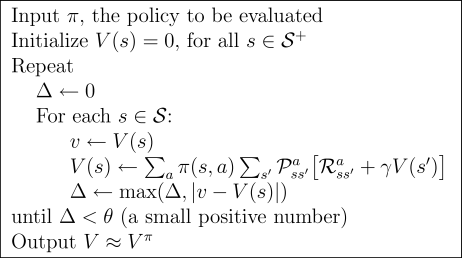
\includegraphics[width=0.7\textwidth]{Grafiken/21pe.png}
    \caption{Pseudocode des Policy-Evaluation Algorithmus}
    \label{fig:policyevaluation}
\end{figure}

\subsection{Policy Improvement}
Grund für das Ermitteln einer Wertfunktion, ist das Bestreben eine bessere Strategie zu finden. Wenn $V^\pi$ eine beliebige Wertfunktion für die  Strategie $\pi$ ist,  ist es interessant, ob für einen Zustand $s$ eine andere Aktion $a\neq\pi(s)$   gewählt werden soll, oder aber die alte Aktion $a=\pi(s)$ beibehalten werden soll.
Es gibt verschiedene Möglichkeiten, diese  Entscheidung zu treffen. Eine ist, eine beliebige Aktion $a$ zu wählen und dann mit der bestehenden Strategie $\pi$ fortzufahren. Der Wert durch Ausführen dieses Aktion $a$ ist durch $Q^\pi(s,a)$ beschrieben. Die Frage, die sich stellt, ist: Ist $Q^\pi(s,a)$ besser als $V^\pi(s)$?
Ist dies der Fall, sollte die ermittelte Aktion $a$ der bestehenden Strategie vorgezogen werden.

Seien $\pi$ und $\pi'$ ein beliebiges Paar von Strategien, so dass für alle $s \in S$ gilt:
\begin{align}
Q^\pi(s,\pi'(s)) \ge V^\pi(s)
\end{align}

Dann ist Strategie $\pi'$  mindestens so gut wie $\pi$, was wiederum bedeutet:

\begin{align}
V^{\pi'}(s) \ge V^\pi(s)
\end{align}

Mathematisch ausgedrückt kann die beste Aktion $a$ für den Zustand $s$ folgendermaßen gefunden werden:

\begin{align}\label{policy-improvement}
\pi'(s) &= arg\underset{a}{max}\sum_{s'}\mathcal{P}^a_{ss'}[\mathcal{R}^a_{ss'}+\gamma V^\pi(s')]
\end{align}

Die Funktion $argmax$ gibt gibt den Funktionsparameter zurück, für den die Funktion den höchsten Wert ergibt\footnote{Z.B. wenn $f(1)=10, f(2) = 50, f(3) = 25$ dann würde $arg\underset{x}{max}f(x)$ den Wert $2$ zurückliefern}. In Gleichung \ref{policy-improvement} wird somit das $a$ zurückgeben, was den höchsten Wert ergibt und so eine Strategie-Verbesserung erreicht. $\pi'$ stellt die verbesserte Strategie dar.

\subsection{Policy Iteration}
Falls sich die Strategie beim Strategie-Verbesserungsschritt (``Policy Improvement'') ändert muss diese neu ausgewertet werden. Somit müssen die V-Werte neu berechnet werden, da sie sich möglicherweise verändert haben.

Hieraus ergibt sich ein Verfahren mit dem schrittweise eine verbesserte Strategie gefunden werden kann. Es wird ausgehend von einer Strategie $\pi_0$ durch abwechselndes Ausführen des Evaluationsschrittes (E) und Verbesserungsschrittes (I) eine bessere Strategie $\pi_1$ berechnet. Im Evaluationsschritt werden die verbesserten $V^{\pi_0}$ Werte berechnet, aus denen dann die Verbesserte Strategie im Verbesserungsschritt abgeleitet wird. Das Verfahren kann durch  folgenden Ausdruck veranschaulicht werden:
\begin{align}
\pi_0 \overset{E}{\longrightarrow} V^{\pi_0} \overset{I}{\longrightarrow} \pi_1 \overset{E}{\longrightarrow} V^{\pi_1} \overset{I}{\longrightarrow} \pi_2  \overset{E}{\longrightarrow} V^{\pi_2} \overset{I}{\longrightarrow} ... \pi^*
\end{align}

Das Verfahren terminiert sofern sich die Strategie beim Verbesserungsschritt nicht mehr verändert.

\subsection{Value Iteration}
Eine wichtige Frage für die Laufzeit und Performanz des Verfahrens wie häufig bei der Strategie-Evaluation über die Bellman-Gleichung iteriert werden soll. Es ist durchaus denkbar, dass bereits nicht besonders exakte V-Werte zu einer Verbesserung der Strategie führen.

Der Ansatz der ``Value Iteration'' besteht darin nur eine Iteration der Bellman-Gleichung im Evalutaionsschritt und direkt darauf folgend eine Strategie-Verbesserung durchzuführen.
Die folgenden beiden Schritte werden abwechselnd durchgeführt (Gleichung \ref{valueiteration1} ist die Strategie Evaluation, Gleichung \ref{valueiteration2} ist die Strategie Verbesserung).
\begin{align}\label{valueiteration1}
V^\pi_{k+1}(s) &= \sum\limits_{a} \pi_{k+1}(s,a) \sum\limits_{s'}\mathcal{P}^a_{ss'}[\mathcal{R}^a_{ss'}+\gamma V^\pi_k(s')]\\
\pi_{k+1}(s) &= arg\underset{a}{max}\sum_{s'}\mathcal{P}^a_{ss'}[\mathcal{R}^a_{ss'}+\gamma V^\pi(s')]\label{valueiteration2}
\end{align}

Die beiden Gleichungen werden zu einer Gleichung zusammengefasst:
\begin{align}
V_{k+1}(s) &= \underset{a}{max}\sum\mathcal{P}^a_{ss'}[\mathcal{R}^a_{ss'}+\gamma V^\pi(s')]
\end{align}
Die Funktion $max$ gibt den besten Wert zurück, der mit einem Parameter a erreicht werden kann\footnote{Z.B. wenn $f(1)=10, f(2)=50, f(3) = 25$ dann würde $\underset{x}{max}$ den Wert $50$ zurückgeben}. Als Abbruchkriterien wird wieder wie bei der ``Policy Evaluation'' die Unterschreitung eines bestimmten Schwellenwertes festgelegt: 
\begin{align}
\max\limits_{s\in S^+} |V_{k+1}(s)-V_k(s)|
\end{align}
In der Abbildung \ref{fig:valueiteration} ist der Pseudocode des ``Value Itation''-Algorithmus aufgeführt.
\begin{figure}[htc]
    \centering
    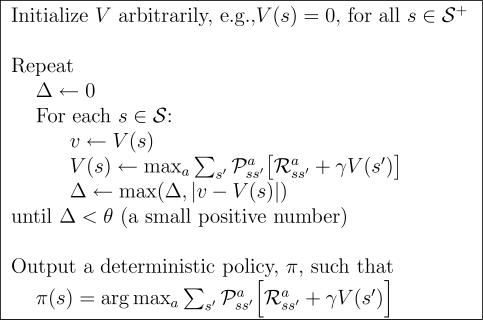
\includegraphics[width=0.7\textwidth]{Grafiken/24vi.png}
    \caption{Pseudocode des Value-Iteration Algorithmus}
    \label{fig:valueiteration}
\end{figure}

\section{Temporal Difference Learning}
Temporal Difference Learning (TD-Learning) beschreibt eine Klasse von Verfahren, die ein Lernen allein aus Erfahrungen ermöglicht. 

Bei der Methode wird versucht die Zustands-Wertfunktion (V-Funktion) zu verbessern. Dazu wird davon ausgegangen, dass der Agent bereits eine vorläufige V-Funktion besitzt, welche aber noch nicht der Wirklichkeit entspricht. Weiterhin müssen Erfahrungen in der Bewertung von zurückliegenden Zuständen einfliessen, da Erfahrungen womöglich erst nach einiger Zeit "zu Tage treten". Somit ist davon auszugehen, dass die Wertfunktion in späteren Zuständen schon näher an der Wirklichkeit liegt. Da jedoch bis zur vollständigen Exploration der Umgebung die V-Funktion von der tatsächlichen Wertefunktion abweicht, wird diese geschätzt.
Dies wird durch folgende Formel spezifiziert:
\begin{equation}
V^\pi = E_\pi{r_{t+1}+\gamma V^ \pi(s_{t+1})}
\end{equation}

Die Zustands-Wertefunktion V für die Strategie $\pi$ ist gleich dem Erwartungswert für den zu erwartenden Gewinn $r_{t+1}$ und der über den Trace-Decay-Faktor verminderten V-Funktion des Folgezustands.

Der Trace-Decay-Faktor ($\gamma$) beschreibt, wie groß die Gewichtung von zukünftigen Entscheidungen ist. Dadurch werden nähere Zustände höher bewertet als spätere, bzw. zukünftige Belohnungen werden schwächer bewertet. Ist der Trace-Decay-Faktor  gleich 1, so entspricht das TD-Learning der Monte-Carlo-Methode.

Weiterhin gibt es noch einen $\alpha$-Wert, welcher angibt, wie nah der Folgewert an dem V-Wert des jetztigen Zustands annähert.Für hinreichend kleine $\alpha$ nähert sich die Methode dem korrektem V-Wert. Somit indiziert $\alpha$ die Lernrate zur Steuerung der Korrekturstärke, also in welchem Maße die Funktion verbessert oder geändert wird.

\subsection{Gierige Wahl von Aktionen}
Eine Strategie heißt gierieg (greedy), wenn sie immer versucht die Aktion zu wählen, die zu einer optimalen Wertefunktion führt. Daraus resultiert das Problem, dass manche Aktionen nicht ausgeführt werden, obwohl die Erfahrung langfristig zeigen würde, dass sie eigentlich besser wären. 
Es ist natürlich nicht sinnvoll einen Agenten zufällig agieren zu lassen und ihn nicht auf seine Erfahrungen zurückgreifen zu lassen. Deshalb wird der Parameter $\varepsilon$ eingeführt, welcher angibt, wie häufig nicht optimale Aktionen ausgewählt werden. Für $\varepsilon = 0$ ist die Strategie gierig, sonst nennt man sie $\varepsilon$-gierig. Meist wird ein konstanter, kleiner $\varepsilon$-Wert gewählt. 

\subsection{On-Policy TD und Off-Policy TD}
On-Policy und Off-Policy TD sind Strategiverbesserungsverfahren, die TD-Learning einsetzen(sic!).

Bei On-Policy TD(SARSA) wird der nächste Zustand anhand eines Pfades berechnet. Falls zufällig durch $\epsilon$ ein nicht optimaler Pfad gewählt wird, kann ein Zustand möglicherweise komplett ausscheiden, obwohl er für die Zielerreichung essentiell wäre. 
\begin{equation}
Q(s_t,a_t) \leftarrow Q(s_t,a_t) + \alpha[r_{t+1}+\gamma Q(s_{t+1},a_{t+1})- Q(s_t,a_t)]
\end{equation}

Die Verbesserung der Q Funktion setzt sich hierbei aus dem alten Funktionswert plus einen durch $\alpha$ abgeschwächten Wert, der aus der zu erwartender Belohnung, sowie der Differenz zwischen Erwartungswert des nächsten und dieses Zustands.

Im Gegensatz dazu wird beim Off-Policy TD die Werteberechnung des nächsten Zustands nicht nur entsprechend eines Pfades durchgeführt, sonder jeweils immer der beste Nachfolgezustand einbezogen. 
Die Formel ändert sich hier nur im letzten Teil:
\begin{equation}
Q(s_t,a_t) \leftarrow Q(s_t,a_t) + \alpha[r_{t+1}+\gamma  \max_\alpha Q(s_{t+1},a)- Q(s_t,a_t)]
\end{equation}

\begin{figure}[htc]
    \centering
    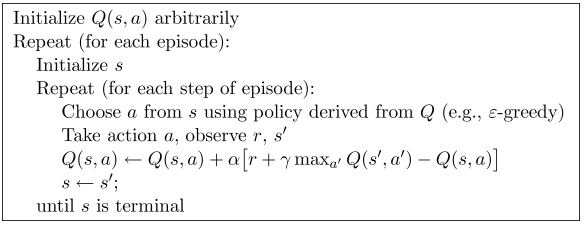
\includegraphics[width=0.7\textwidth]{Grafiken/ql.png}
    \caption{Pseudocode Q-Learning}
    \label{fig:qlearning}
\end{figure}

\begin{figure}[htc]
    \centering
    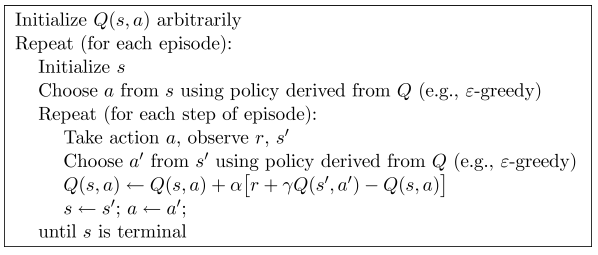
\includegraphics[width=0.7\textwidth]{Grafiken/sarsa.png}
    \caption{Pseudocode Sarsa}
    \label{fig:sarsa}
\end{figure}

Die Algorithmen für Sarsa und Q-Learning sind in Abbildung \ref{fig:sarsa} und \ref{fig:qlearning} zu sehen \cite{krl}.

Um den Unterschied zwischen dem On-Policy und Off-Policy Verfahren zu verdeutlichen, führt Sutton und Barto \cite{rli} das Beipsiel einer Cliff-Anwendung (Abbildung \ref{fig:cliff}) an. Hier soll ein Weg von S zu G zurückgelegt werden. Alle Felder haben die Belohnung $-1$, bis auf das Cliff, hier ist der Wert $-100$. Da Q-Learning immer die optimale Aktion wählt, wählt ein Agent mit diesem Verfahren einen Weg direkt am Cliff entlang. Er stürtzt durch den $\varepsilon$-Wert nur selten ab. Beim Sarsa Verfahren bedingt die Aktionsauswahl den Weg. Hierzu kommt es zu häufigeren Abstürzen und der Agent wählt den sichersten Weg. Würde das $\varepsilon$ kleiner werden, würden beide Verfahren den optimalen Weg wählen.

\begin{figure}[htc]
    \centering
    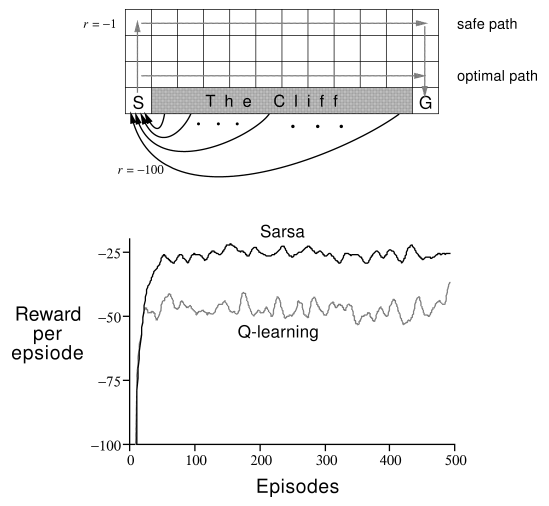
\includegraphics[width=0.7\textwidth]{Grafiken/cliff.png}
    \caption{Cliff-Anwendung \cite{rli}}
    \label{fig:cliff}
\end{figure}

\section{Fazit}
Das Szenario des Krabbelroboter fordert vom eingesetzten Verfahren eine kontinuierliche Arbeitsweise und nicht vollständiges Wissen über die Umwelt. Durch die Anforderung des nicht vollständigen Wissens scheidet die Dynamische Programmierung aus. Die Monte Carlo Methode wartet bis zum Ende einer Episode um Informationen über die Belohnung zu erhalten, dies widerspricht der Anforderung der Kontinuität. Temproal Difference Learning bietet beide Eigenschaften. Hier ist die Off-Policy Variante mit einem hohen $\epsilon$ zu wählen, um auf eventuell Auftretende Hindernisse zu reagieren.

\bibliographystyle{dinat}
\bibliography{bericht}

\end{document}

